\documentclass[class=report, crop=false, 12pt,a4paper]{standalone}
\usepackage{enumitem}
\usepackage{multicol}
\usepackage{graphicx}
\usepackage{float}
\usepackage{amsmath}
\usepackage{amssymb}
\usepackage{mathtools}
\usepackage{siunitx}
\usepackage{commath}
\usepackage{array}
\usepackage{natbib}
\usepackage{tikz}
\usepackage[a4paper,width=150mm,top=25mm,bottom=25mm]{geometry}
\usetikzlibrary{positioning, fit, calc}   
\tikzset{block/.style={draw, thick, text width=3cm ,minimum height=1.3cm, align=center},   
line/.style={-latex}     
}  
\setlength{\parindent}{0pt}
\begin{document}
\section{Conformal mapping}
\subsection{Joukowsky Transformation}
The question is how can we transform our cylinder into something that looks like an airfoil? We achieve this by using conformal mapping which maps each part of our coordinate space to a new one. 
\begin{align}
  x &= r\cos{\theta}\\
  y &= r\sin{\theta}\\
  w &= G(z) = z + \frac{\lambda^2}{z}\\
  z &= re^{i\theta} = x + yi\\
  w &= \zeta + \xi i
\end{align}
\begin{figure}[H]
  \centering
  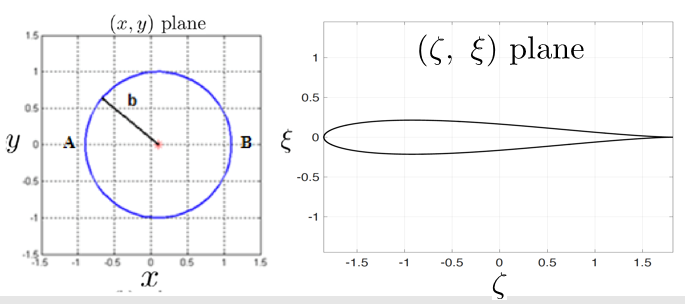
\includegraphics[width = 0.9\textwidth]{../img/diagram32.png}
\end{figure}
\subsection{Flat plate and Ellipse}
Lets consider a cylinder:
\begin{figure}[H]
  \centering
  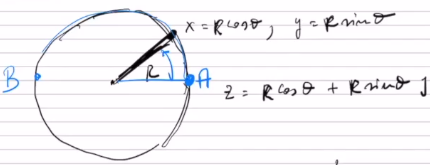
\includegraphics[width = 0.9\textwidth]{../img/diagram33.png}
\end{figure}
\begin{align}
  z &= R\cos{\theta} + Ri\sin{\theta}\\
  w &= G(z) = z + \frac{\lambda^2}{z}\\
  &=  R\cos{\theta} + Ri\sin{\theta} + \frac{\lambda^2}{R\cos{\theta} + Ri\sin{\theta}}\\
  &= R\cos{\theta} + Ri\sin{\theta} + \frac{\lambda^2 (R\cos{\theta} - Ri\sin{\theta})}{(R\cos{\theta} + Ri\sin{\theta})(R\cos{\theta} - Ri\sin{\theta})}\\
  &= R\cos{\theta} + Ri\sin{\theta} + \frac{\lambda^2 (R\cos{\theta} - Ri\sin{\theta})}{R^2}\\
  w &= R\cos{\theta} \left(1 + \frac{\lambda^2}{R}\right) + Ri\sin{\theta} \left(1 - \frac{\lambda^2}{R}\right)
\end{align}
When $\lambda = R$, we achieve a flat plate transformation as our imaginary term is always 0. When $\lambda \neq R$, we achieve an elliptical shape.
\begin{figure}[H]
  \centering
  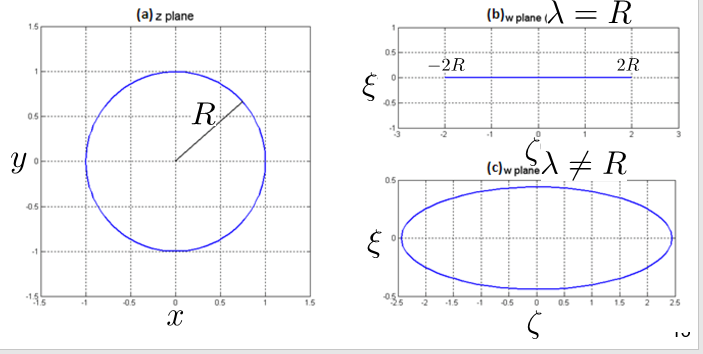
\includegraphics[width = 0.9\textwidth]{../img/diagram34.png}
\end{figure}
\end{document}